\PassOptionsToPackage{unicode=true}{hyperref} % options for packages loaded elsewhere
\PassOptionsToPackage{hyphens}{url}
%
\documentclass[ignorenonframetext,]{beamer}
\usepackage{pgfpages}
\setbeamertemplate{caption}[numbered]
\setbeamertemplate{caption label separator}{: }
\setbeamercolor{caption name}{fg=normal text.fg}
\beamertemplatenavigationsymbolsempty
\usepackage{lmodern}
\usepackage{amssymb,amsmath}
\usepackage{ifxetex,ifluatex}
\usepackage{fixltx2e} % provides \textsubscript
\ifnum 0\ifxetex 1\fi\ifluatex 1\fi=0 % if pdftex
  \usepackage[T1]{fontenc}
  \usepackage[utf8]{inputenc}
  \usepackage{textcomp} % provides euro and other symbols
\else % if luatex or xelatex
  \usepackage{unicode-math}
  \defaultfontfeatures{Ligatures=TeX,Scale=MatchLowercase}
\fi
\usetheme[]{CambridgeUS}
\usecolortheme{beaver}
\usefonttheme{structurebold}
% use upquote if available, for straight quotes in verbatim environments
\IfFileExists{upquote.sty}{\usepackage{upquote}}{}
% use microtype if available
\IfFileExists{microtype.sty}{%
\usepackage[]{microtype}
\UseMicrotypeSet[protrusion]{basicmath} % disable protrusion for tt fonts
}{}
\IfFileExists{parskip.sty}{%
\usepackage{parskip}
}{% else
\setlength{\parindent}{0pt}
\setlength{\parskip}{6pt plus 2pt minus 1pt}
}
\usepackage{hyperref}
\hypersetup{
            pdftitle={A7 Die R-Pakete sp und spdep},
            pdfauthor={Jan-Philipp Kolb},
            pdfborder={0 0 0},
            breaklinks=true}
\urlstyle{same}  % don't use monospace font for urls
\newif\ifbibliography
\usepackage{color}
\usepackage{fancyvrb}
\newcommand{\VerbBar}{|}
\newcommand{\VERB}{\Verb[commandchars=\\\{\}]}
\DefineVerbatimEnvironment{Highlighting}{Verbatim}{commandchars=\\\{\}}
% Add ',fontsize=\small' for more characters per line
\usepackage{framed}
\definecolor{shadecolor}{RGB}{248,248,248}
\newenvironment{Shaded}{\begin{snugshade}}{\end{snugshade}}
\newcommand{\AlertTok}[1]{\textcolor[rgb]{0.94,0.16,0.16}{#1}}
\newcommand{\AnnotationTok}[1]{\textcolor[rgb]{0.56,0.35,0.01}{\textbf{\textit{#1}}}}
\newcommand{\AttributeTok}[1]{\textcolor[rgb]{0.77,0.63,0.00}{#1}}
\newcommand{\BaseNTok}[1]{\textcolor[rgb]{0.00,0.00,0.81}{#1}}
\newcommand{\BuiltInTok}[1]{#1}
\newcommand{\CharTok}[1]{\textcolor[rgb]{0.31,0.60,0.02}{#1}}
\newcommand{\CommentTok}[1]{\textcolor[rgb]{0.56,0.35,0.01}{\textit{#1}}}
\newcommand{\CommentVarTok}[1]{\textcolor[rgb]{0.56,0.35,0.01}{\textbf{\textit{#1}}}}
\newcommand{\ConstantTok}[1]{\textcolor[rgb]{0.00,0.00,0.00}{#1}}
\newcommand{\ControlFlowTok}[1]{\textcolor[rgb]{0.13,0.29,0.53}{\textbf{#1}}}
\newcommand{\DataTypeTok}[1]{\textcolor[rgb]{0.13,0.29,0.53}{#1}}
\newcommand{\DecValTok}[1]{\textcolor[rgb]{0.00,0.00,0.81}{#1}}
\newcommand{\DocumentationTok}[1]{\textcolor[rgb]{0.56,0.35,0.01}{\textbf{\textit{#1}}}}
\newcommand{\ErrorTok}[1]{\textcolor[rgb]{0.64,0.00,0.00}{\textbf{#1}}}
\newcommand{\ExtensionTok}[1]{#1}
\newcommand{\FloatTok}[1]{\textcolor[rgb]{0.00,0.00,0.81}{#1}}
\newcommand{\FunctionTok}[1]{\textcolor[rgb]{0.00,0.00,0.00}{#1}}
\newcommand{\ImportTok}[1]{#1}
\newcommand{\InformationTok}[1]{\textcolor[rgb]{0.56,0.35,0.01}{\textbf{\textit{#1}}}}
\newcommand{\KeywordTok}[1]{\textcolor[rgb]{0.13,0.29,0.53}{\textbf{#1}}}
\newcommand{\NormalTok}[1]{#1}
\newcommand{\OperatorTok}[1]{\textcolor[rgb]{0.81,0.36,0.00}{\textbf{#1}}}
\newcommand{\OtherTok}[1]{\textcolor[rgb]{0.56,0.35,0.01}{#1}}
\newcommand{\PreprocessorTok}[1]{\textcolor[rgb]{0.56,0.35,0.01}{\textit{#1}}}
\newcommand{\RegionMarkerTok}[1]{#1}
\newcommand{\SpecialCharTok}[1]{\textcolor[rgb]{0.00,0.00,0.00}{#1}}
\newcommand{\SpecialStringTok}[1]{\textcolor[rgb]{0.31,0.60,0.02}{#1}}
\newcommand{\StringTok}[1]{\textcolor[rgb]{0.31,0.60,0.02}{#1}}
\newcommand{\VariableTok}[1]{\textcolor[rgb]{0.00,0.00,0.00}{#1}}
\newcommand{\VerbatimStringTok}[1]{\textcolor[rgb]{0.31,0.60,0.02}{#1}}
\newcommand{\WarningTok}[1]{\textcolor[rgb]{0.56,0.35,0.01}{\textbf{\textit{#1}}}}
\usepackage{graphicx,grffile}
\makeatletter
\def\maxwidth{\ifdim\Gin@nat@width>\linewidth\linewidth\else\Gin@nat@width\fi}
\def\maxheight{\ifdim\Gin@nat@height>\textheight\textheight\else\Gin@nat@height\fi}
\makeatother
% Scale images if necessary, so that they will not overflow the page
% margins by default, and it is still possible to overwrite the defaults
% using explicit options in \includegraphics[width, height, ...]{}
\setkeys{Gin}{width=\maxwidth,height=\maxheight,keepaspectratio}
% Prevent slide breaks in the middle of a paragraph:
\widowpenalties 1 10000
\raggedbottom
\setbeamertemplate{part page}{
\centering
\begin{beamercolorbox}[sep=16pt,center]{part title}
  \usebeamerfont{part title}\insertpart\par
\end{beamercolorbox}
}
\setbeamertemplate{section page}{
\centering
\begin{beamercolorbox}[sep=12pt,center]{part title}
  \usebeamerfont{section title}\insertsection\par
\end{beamercolorbox}
}
\setbeamertemplate{subsection page}{
\centering
\begin{beamercolorbox}[sep=8pt,center]{part title}
  \usebeamerfont{subsection title}\insertsubsection\par
\end{beamercolorbox}
}
\AtBeginPart{
  \frame{\partpage}
}
\AtBeginSection{
  \ifbibliography
  \else
    \frame{\sectionpage}
  \fi
}
\AtBeginSubsection{
  \frame{\subsectionpage}
}
\setlength{\emergencystretch}{3em}  % prevent overfull lines
\providecommand{\tightlist}{%
  \setlength{\itemsep}{0pt}\setlength{\parskip}{0pt}}
\setcounter{secnumdepth}{0}

% set default figure placement to htbp
\makeatletter
\def\fps@figure{htbp}
\makeatother


\title{A7 Die R-Pakete \texttt{sp} und \texttt{spdep}}
\author{Jan-Philipp Kolb}
\date{22 Oktober 2018}

\begin{document}
\frame{\titlepage}

\begin{frame}{Themen dieses Abschnitts}
\protect\hypertarget{themen-dieses-abschnitts}{}

\begin{itemize}
\tightlist
\item
  Eine räumliche Stichprobe ziehen
\item
  Adressen für die gezogenen Punkte bestimmen
\item
  Adressdatensatz bereinigen
\item
  Wie lässt sich die Entfernung bestimmen
\end{itemize}

\begin{block}{Das erste Gesetz der Geographie (TFLG)}

\begin{quote}
``All things are related, but nearby things are more related than
distant things'' {[}Tobler, 1970{]}
\end{quote}

\end{block}

\end{frame}

\begin{frame}[fragile]{\href{http://www.geodatenzentrum.de/geodaten/gdz_rahmen.gdz_div?gdz_spr=deu\&gdz_akt_zeile=5\&gdz_anz_zeile=1\&gdz_unt_zeile=13\&gdz_user_id=0}{Shapefile
mit Regionalschlüssel} herunterladen}
\protect\hypertarget{shapefile-mit-regionalschlussel-herunterladen}{}

\begin{Shaded}
\begin{Highlighting}[]
\KeywordTok{library}\NormalTok{(rgdal)}
\end{Highlighting}
\end{Shaded}

\begin{verbatim}
## Loading required package: sp
\end{verbatim}

\begin{verbatim}
## rgdal: version: 1.3-2, (SVN revision 755)
##  Geospatial Data Abstraction Library extensions to R successfully loaded
##  Loaded GDAL runtime: GDAL 2.2.3, released 2017/11/20
##  Path to GDAL shared files: D:/Eigene Dateien/Dokumente/R/win-library/3.5/rgdal/gdal
##  GDAL binary built with GEOS: TRUE 
##  Loaded PROJ.4 runtime: Rel. 4.9.3, 15 August 2016, [PJ_VERSION: 493]
##  Path to PROJ.4 shared files: D:/Eigene Dateien/Dokumente/R/win-library/3.5/rgdal/proj
##  Linking to sp version: 1.3-1
\end{verbatim}

\begin{Shaded}
\begin{Highlighting}[]
\KeywordTok{setwd}\NormalTok{(vg250path)}
\NormalTok{VG250 <-}\StringTok{ }\KeywordTok{readOGR}\NormalTok{ (}\StringTok{"VG250_GEM.shp"}\NormalTok{,}\StringTok{"VG250_GEM"}\NormalTok{)}
\end{Highlighting}
\end{Shaded}

\begin{verbatim}
## OGR data source with driver: ESRI Shapefile 
## Source: "D:\GESIS\data\vg250_3112.utm32s.shape.ebenen\vg250_ebenen\VG250_GEM.shp", layer: "VG250_GEM"
## with 11395 features
## It has 23 fields
\end{verbatim}

\end{frame}

\begin{frame}[fragile]{\href{https://www.rdocumentation.org/packages/sp/versions/1.3-1/topics/spsample}{Räumliche
Stichprobe}}
\protect\hypertarget{raumliche-stichprobe}{}

\begin{itemize}
\tightlist
\item
  Mit der Funktion \texttt{spsample} aus dem Paket \texttt{sp} kann man
  eine räumliche Stichprobe ziehen.
\end{itemize}

\begin{Shaded}
\begin{Highlighting}[]
\NormalTok{spatsamp <-}\StringTok{ }\KeywordTok{spsample}\NormalTok{(VG250, }\DecValTok{100}\NormalTok{,}\DataTypeTok{type=}\StringTok{"random"}\NormalTok{)}
\end{Highlighting}
\end{Shaded}

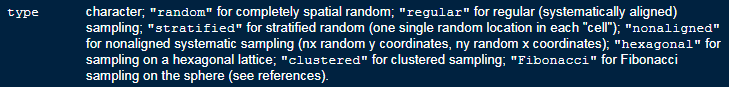
\includegraphics{figure/spsample_type.PNG}

\end{frame}

\begin{frame}[fragile]{Point in Polygon}
\protect\hypertarget{point-in-polygon}{}

\begin{itemize}
\tightlist
\item
  Mit der Funktion \texttt{over} kann man feststellen in welchem Polygon
  ein Punkt liegt.
\end{itemize}

\begin{Shaded}
\begin{Highlighting}[]
\NormalTok{tmp <-}\StringTok{ }\NormalTok{sp}\OperatorTok{::}\KeywordTok{over}\NormalTok{(spatsamp, VG250)}
\end{Highlighting}
\end{Shaded}

\begin{Shaded}
\begin{Highlighting}[]
\KeywordTok{head}\NormalTok{(tmp)}
\end{Highlighting}
\end{Shaded}

\begin{verbatim}
##   ADE GF BSG           RS      AGS       SDV_RS       GEN      BEZ IBZ
## 1   6  4   1 120695904052 12069052 120695904052 Borkheide Gemeinde  64
## 2   6  4   1 147300180180 14730180 147300180180  Löbnitz Gemeinde  62
## 3   6  4   1 160755004063 16075063 160755004063    Löhma Gemeinde  64
## 4   6  4   1 092785248134 09278134 092785248134 Haselbach Gemeinde  64
## 5   6  4   1 034600003003 03460003 034600003003  Dinklage    Stadt  61
## 6   6  4   1 032410017017 03241017 032410017017   Springe    Stadt  61
##                       BEM NBD SN_L SN_R SN_K SN_V1 SN_V2 SN_G FK_S3  NUTS
## 1 gemeinschaftsangehörig  ja   12    0   69    59    04  052     R DE40E
## 2                      --  ja   14    7   30    01    80  180     K DED53
## 3 gemeinschaftsangehörig  ja   16    0   75    50    04  063     R DEG0K
## 4 gemeinschaftsangehörig  ja   09    2   78    52    48  134     R DE22B
## 5                      --  ja   03    4   60    00    03  003     K DE94F
## 6                      --  ja   03    2   41    00    17  017     K DE929
##           RS_0    AGS_0        WSK         DEBKG_ID
## 1 120695904052 12069052 2009/01/01 DEBKGDL20000E3FZ
## 2 147300180180 14730180 2009/01/01 DEBKGDL20000DYEX
## 3 160755004063 16075063 2009/01/01 DEBKGDL20000DVXD
## 4 092785248134 09278134 1978/05/01 DEBKGDL20000E4PJ
## 5 034600003003 03460003 2009/01/01 DEBKGDL20000E1PD
## 6 032410017017 03241017 2009/01/01 DEBKGDL20000E6SJ
\end{verbatim}

\end{frame}

\begin{frame}[fragile]{Daten in ein anderes CRS übertragen}
\protect\hypertarget{daten-in-ein-anderes-crs-ubertragen}{}

\begin{Shaded}
\begin{Highlighting}[]
\KeywordTok{library}\NormalTok{(sp)}
\end{Highlighting}
\end{Shaded}

\begin{quote}
spTransform for map projection and datum transformation
\end{quote}

\begin{Shaded}
\begin{Highlighting}[]
\CommentTok{# EPSG: 3857}
\NormalTok{newData<-sp}\OperatorTok{::}\KeywordTok{spTransform}\NormalTok{(spatsamp, }\KeywordTok{CRS}\NormalTok{(}\StringTok{"+init=epsg:3857"}\NormalTok{))}
\end{Highlighting}
\end{Shaded}

\end{frame}

\begin{frame}[fragile]{Eine Karte von Afrika}
\protect\hypertarget{eine-karte-von-afrika}{}

\begin{Shaded}
\begin{Highlighting}[]
\KeywordTok{library}\NormalTok{(maptools)}
\KeywordTok{data}\NormalTok{(wrld_simpl)}
\NormalTok{Africa <-}\StringTok{ }\NormalTok{wrld_simpl[wrld_simpl}\OperatorTok{@}\NormalTok{data}\OperatorTok{$}\NormalTok{REGION}\OperatorTok{==}\DecValTok{2}\NormalTok{,]}
\KeywordTok{plot}\NormalTok{(Africa)}
\end{Highlighting}
\end{Shaded}

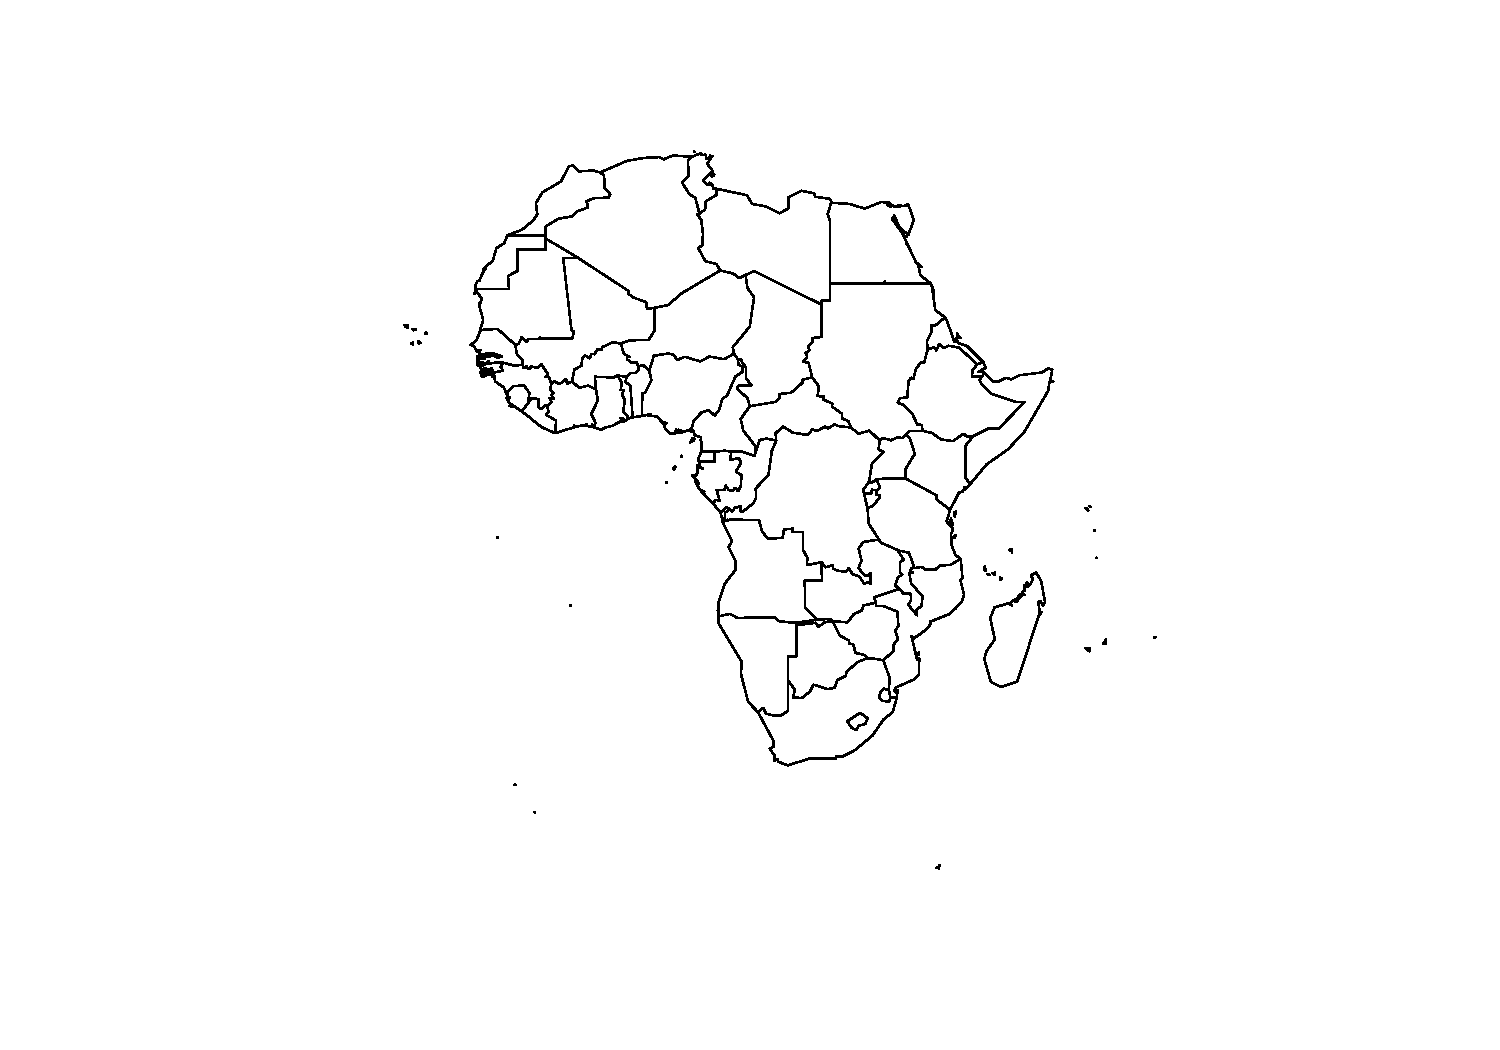
\includegraphics{A7_spdep_files/figure-beamer/unnamed-chunk-10-1.pdf}

\end{frame}

\begin{frame}[fragile]{Das Zentrum eines Polygonzuges}
\protect\hypertarget{das-zentrum-eines-polygonzuges}{}

\begin{Shaded}
\begin{Highlighting}[]
\NormalTok{Af <-}\StringTok{ }\KeywordTok{coordinates}\NormalTok{(Africa)}
\KeywordTok{head}\NormalTok{(Af)}
\end{Highlighting}
\end{Shaded}

\begin{verbatim}
##          [,1]        [,2]
## DZA  2.627813  28.1721102
## AGO 17.552463 -12.3503789
## BEN  2.332296   9.6047655
## COG 15.218362  -0.8732659
## COD 23.646032  -2.8711605
## BDI 29.901786  -3.3461606
\end{verbatim}

\end{frame}

\begin{frame}[fragile]{Die Koordinaten plotten}
\protect\hypertarget{die-koordinaten-plotten}{}

\begin{Shaded}
\begin{Highlighting}[]
\KeywordTok{plot}\NormalTok{(Africa)}
\KeywordTok{points}\NormalTok{(}\DataTypeTok{x=}\NormalTok{Af[}\DecValTok{1}\NormalTok{,}\DecValTok{1}\NormalTok{],}\DataTypeTok{y=}\NormalTok{Af[}\DecValTok{1}\NormalTok{,}\DecValTok{2}\NormalTok{],}\DataTypeTok{col=}\StringTok{"red"}\NormalTok{,}\DataTypeTok{pch=}\DecValTok{20}\NormalTok{)}
\end{Highlighting}
\end{Shaded}

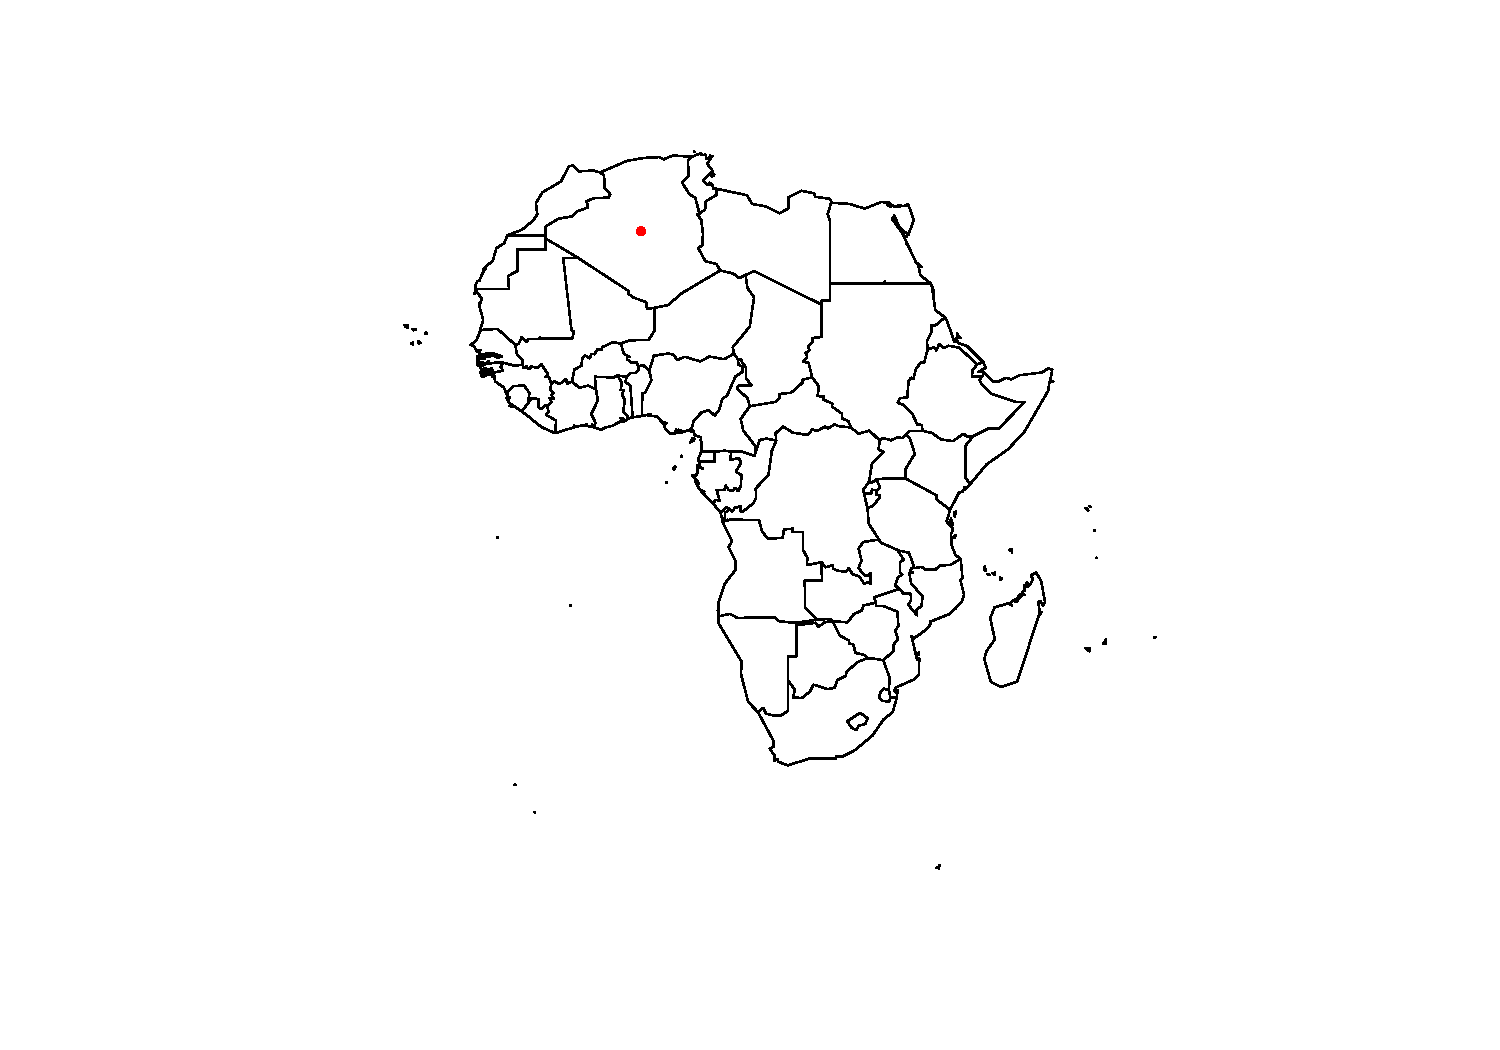
\includegraphics{A7_spdep_files/figure-beamer/unnamed-chunk-12-1.pdf}

\end{frame}

\begin{frame}[fragile]{Die nächsten Nachbarn finden}
\protect\hypertarget{die-nachsten-nachbarn-finden}{}

\begin{Shaded}
\begin{Highlighting}[]
\KeywordTok{library}\NormalTok{(spdep)}
\NormalTok{Af_nb <-}\StringTok{ }\KeywordTok{tri2nb}\NormalTok{(Af)}
\end{Highlighting}
\end{Shaded}

Die Nachbarn für das erste Land:

\begin{Shaded}
\begin{Highlighting}[]
\NormalTok{Af_nb[}\DecValTok{1}\NormalTok{]}
\end{Highlighting}
\end{Shaded}

\begin{verbatim}
## [[1]]
## [1] 24 26 27 32 48
\end{verbatim}

\end{frame}

\begin{frame}[fragile]{Die Nachbarn finden}
\protect\hypertarget{die-nachbarn-finden}{}

\begin{Shaded}
\begin{Highlighting}[]
\KeywordTok{plot}\NormalTok{(Africa)}
\KeywordTok{plot}\NormalTok{(Africa[}\DecValTok{1}\NormalTok{,],}\DataTypeTok{col=}\StringTok{"red"}\NormalTok{,}\DataTypeTok{add=}\NormalTok{T)}
\KeywordTok{plot}\NormalTok{(Africa[Af_nb[}\DecValTok{1}\NormalTok{][[}\DecValTok{1}\NormalTok{]],],}\DataTypeTok{col=}\StringTok{"orange"}\NormalTok{,}\DataTypeTok{add=}\NormalTok{T)}
\end{Highlighting}
\end{Shaded}


\includegraphics{A7_spdep_files/figure-beamer/unnamed-chunk-15-1.pdf}

\end{frame}

\begin{frame}[fragile]{\emph{k nearest neighbours}}
\protect\hypertarget{k-nearest-neighbours}{}

\begin{Shaded}
\begin{Highlighting}[]
\NormalTok{IDs <-}\StringTok{ }\KeywordTok{row.names}\NormalTok{(}\KeywordTok{as}\NormalTok{(Africa, }\StringTok{"data.frame"}\NormalTok{))}
\NormalTok{(Af10_nb <-}\StringTok{ }\KeywordTok{knn2nb}\NormalTok{(}\KeywordTok{knearneigh}\NormalTok{(Af, }\DataTypeTok{k =} \DecValTok{10}\NormalTok{), }\DataTypeTok{row.names =}\NormalTok{ IDs))}
\end{Highlighting}
\end{Shaded}

\begin{verbatim}
## Neighbour list object:
## Number of regions: 57 
## Number of nonzero links: 570 
## Percentage nonzero weights: 17.54386 
## Average number of links: 10 
## Non-symmetric neighbours list
\end{verbatim}

\end{frame}

\begin{frame}[fragile]{Die 10 nächsten Nachbarn finden}
\protect\hypertarget{die-10-nachsten-nachbarn-finden}{}

\begin{Shaded}
\begin{Highlighting}[]
\KeywordTok{plot}\NormalTok{(Africa)}
\KeywordTok{plot}\NormalTok{(Africa[}\DecValTok{1}\NormalTok{,],}\DataTypeTok{col=}\StringTok{"red"}\NormalTok{,}\DataTypeTok{add=}\NormalTok{T)}
\KeywordTok{plot}\NormalTok{(Africa[Af10_nb[}\DecValTok{1}\NormalTok{][[}\DecValTok{1}\NormalTok{]],],}\DataTypeTok{col=}\StringTok{"orange"}\NormalTok{,}\DataTypeTok{add=}\NormalTok{T)}
\end{Highlighting}
\end{Shaded}

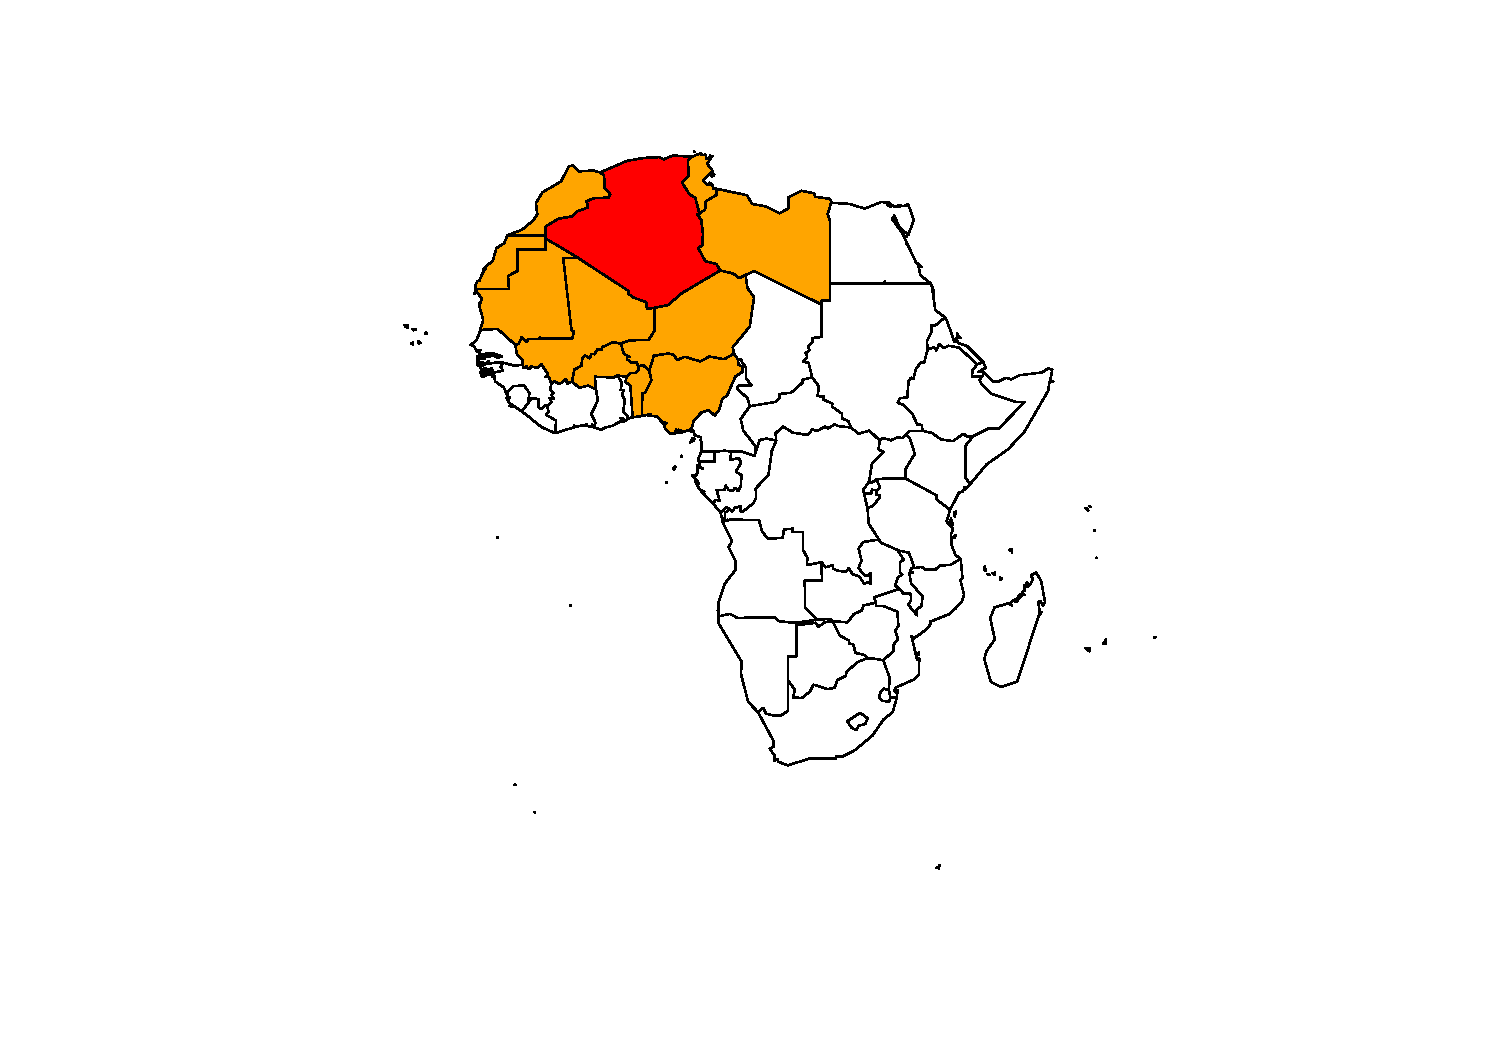
\includegraphics{A7_spdep_files/figure-beamer/unnamed-chunk-17-1.pdf}

\end{frame}

\begin{frame}[fragile]{Die Distanz berechnen}
\protect\hypertarget{die-distanz-berechnen}{}

\begin{Shaded}
\begin{Highlighting}[]
\NormalTok{Af <-}\StringTok{ }\KeywordTok{coordinates}\NormalTok{(Africa) }\CommentTok{# get centroid}
\KeywordTok{library}\NormalTok{(raster)}
\KeywordTok{pointDistance}\NormalTok{(Af[}\DecValTok{1}\OperatorTok{:}\DecValTok{4}\NormalTok{,], }\DataTypeTok{lonlat=}\OtherTok{TRUE}\NormalTok{) }\CommentTok{# compute distance}
\end{Highlighting}
\end{Shaded}

\begin{verbatim}
##         [,1]    [,2]    [,3] [,4]
## [1,]       0      NA      NA   NA
## [2,] 4763231       0      NA   NA
## [3,] 2055609 2954497       0   NA
## [4,] 3484053 1295173 1839191    0
\end{verbatim}

\end{frame}

\begin{frame}[fragile]{Berechnen/zeichnen einer Distanzmatrix}
\protect\hypertarget{berechnenzeichnen-einer-distanzmatrix}{}

\begin{Shaded}
\begin{Highlighting}[]
\NormalTok{Dist_Af <-}\StringTok{ }\KeywordTok{pointDistance}\NormalTok{(Af, }\DataTypeTok{lonlat=}\OtherTok{TRUE}\NormalTok{)}
\NormalTok{Af_color <-}\StringTok{ }\NormalTok{Dist_Af[,}\DecValTok{1}\NormalTok{]}
\NormalTok{Af_color <-}\StringTok{ }\NormalTok{Af_color}\OperatorTok{/}\KeywordTok{max}\NormalTok{(Af_color)}
\NormalTok{Af_color <-}\StringTok{ }\KeywordTok{rgb}\NormalTok{(Af_color,}\DecValTok{0}\NormalTok{,}\DecValTok{0}\NormalTok{)}
\KeywordTok{plot}\NormalTok{(Africa,}\DataTypeTok{col=}\NormalTok{Af_color)}
\end{Highlighting}
\end{Shaded}

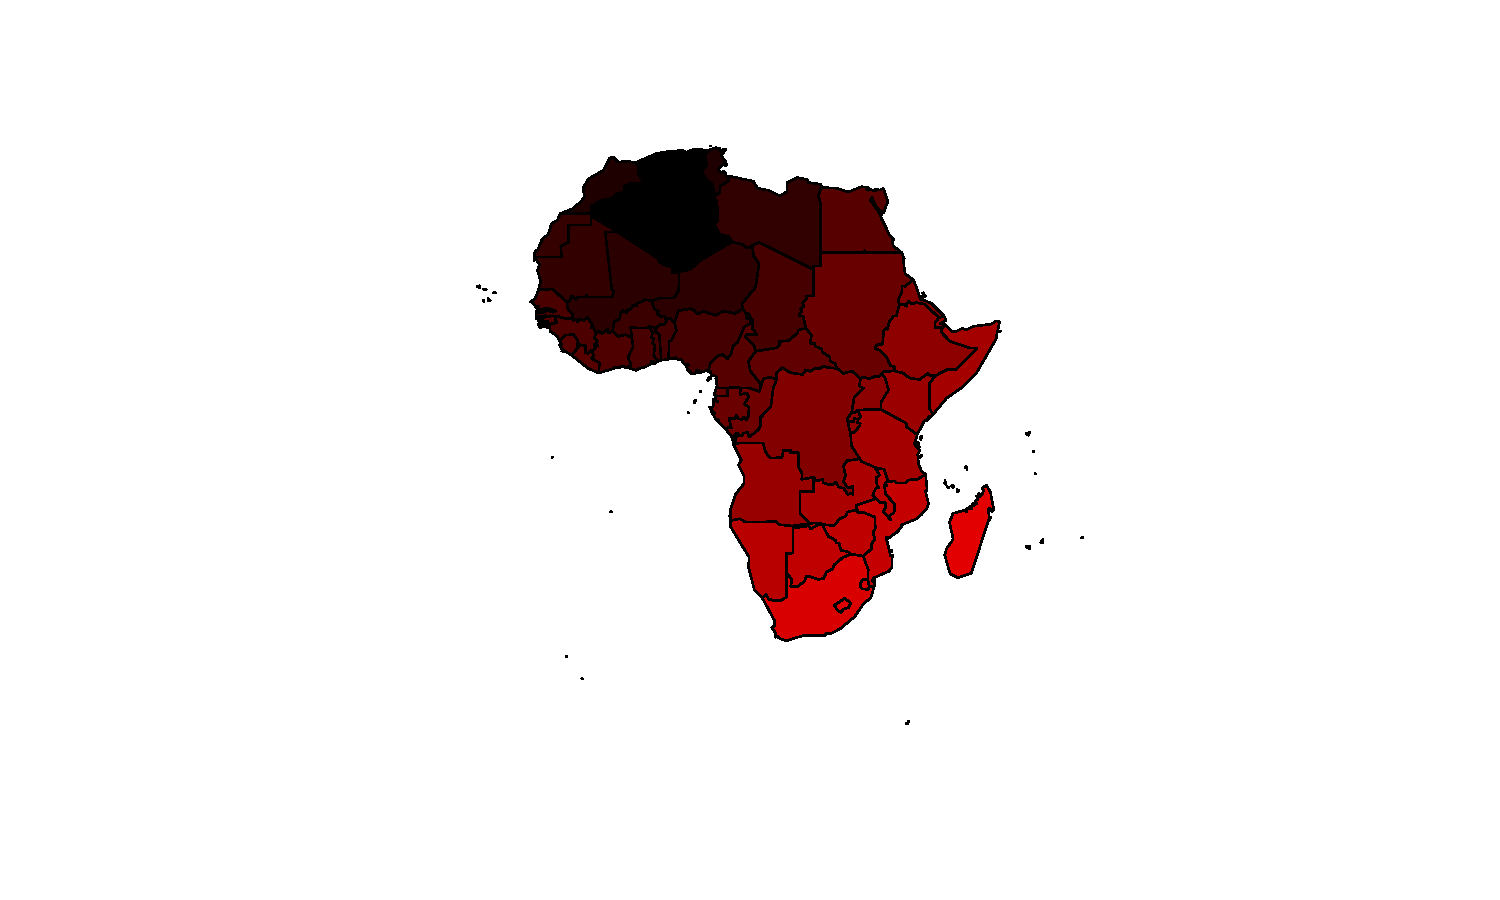
\includegraphics{A7_spdep_files/figure-beamer/Africa Distance-1.pdf}

\end{frame}

\begin{frame}[fragile]{A7A Übung - Nachbarschaften in London}
\protect\hypertarget{a7a-ubung---nachbarschaften-in-london}{}

\begin{itemize}
\tightlist
\item
  Lade den Datensatz london\_sport von meinem Github Verzeichnis
  herunter.
\item
  Importiere den Datensatz.
\item
  Bestimme die nächsten Nachbarn des Stadtteils \emph{City of London}
\end{itemize}

\begin{Shaded}
\begin{Highlighting}[]
\KeywordTok{setwd}\NormalTok{(}\StringTok{"D:/github/geocourse/data/"}\NormalTok{)}
\NormalTok{london_sport <-}\StringTok{ }\KeywordTok{readOGR}\NormalTok{ (}\StringTok{"london_sport.shp"}\NormalTok{,}\StringTok{"london_sport"}\NormalTok{)}
\end{Highlighting}
\end{Shaded}

\begin{verbatim}
## OGR data source with driver: ESRI Shapefile 
## Source: "D:\github\geocourse\data\london_sport.shp", layer: "london_sport"
## with 33 features
## It has 4 fields
## Integer64 fields read as strings:  Pop_2001
\end{verbatim}

\end{frame}

\begin{frame}{Links}
\protect\hypertarget{links}{}

\begin{itemize}
\tightlist
\item
  \href{https://procomun.wordpress.com/2011/06/17/raster-cmsaf-and-solar/}{\textbf{Raster,
  CMSAF and solaR}}
\end{itemize}

\url{https://procomun.wordpress.com/2011/06/17/raster-cmsaf-and-solar/}

\begin{itemize}
\tightlist
\item
  \href{https://johnbaumgartner.wordpress.com/2012/07/26/getting-rasters-into-shape-from-r/}{\textbf{Getting
  rasters into shape from R}}
\end{itemize}

\url{https://johnbaumgartner.wordpress.com/2012/07/26/getting-rasters-into-shape-from-r/}

\end{frame}

\end{document}
